\documentclass[]{spie}  %>>> use for US letter paper
%\documentclass[a4paper]{spie}  %>>> use this instead for A4 paper
%\documentclass[nocompress]{spie}  %>>> to avoid compression of citations

\renewcommand{\baselinestretch}{1.65} % Change to 1.65 for double spacing
\usepackage{listings}
\usepackage{amsmath,amsfonts,amssymb}
\usepackage{graphicx}
\usepackage{upquote}
\usepackage[colorlinks=true, allcolors=blue]{hyperref}

\title{Salisbury University Research Database}

\author{Grant Dawson, Joseph Fernandez, Brock Forsythe, Blaine Mason, Justin Ventura}


% Option to view page numbers
\pagestyle{empty} % change to \pagestyle{plain} for page numbers   
\setcounter{page}{301} % Set start page numbering at e.g. 301
 
\begin{document} 
\maketitle

\section{Motivation}
Salisbury University's Office of Undergraduate Research and Creative Activity(OURCA) has made many attempts to allow students to conduct research at Salisbury.  OURCA's most recently created a data table on the Salisbury University website for current professors who have submitted information regarding their research.  The table has around twenty rows of data so far and just contains contact information and research interests.  We are interested in creating a database focused on the previous and current projects of each faculty member.  One where a professor can have a profile that they are free to add, edit, and remove projects to.  Also, features about a research project such as a poster, paper, or presentation can be displayed as well. Overall, we want to create an effective way to increase the amount of research done at Salisbury University.

Our primary clients are OURCA and research committees within the University.  We would like our database to be accessible from the current "Research Directory" on OURCA's page within Salisbury University's website.  
%to be continued 
\section{Purpose}
One of the main reason students do not get the chance to participate in research projects is the lack of  knowing projects are taking place.  The Salisbury University Research Database will serve as an online tool to assist in the formation of faculty advised research projects. With this in mind, we want to provide a user friendly interface for research seeking students.  Our database will be open to every major and subject of research at Salisbury University.  

The database will serve as a container for current and old research projects at Salisbury.  Each faculty member will have a login on the site and can create a profile. This is where past and current projects, research statement, availability, contact, and funding information will be located.
\newpage
\section{Requirements}
\begin{itemize}
    \item Our database keeps track of a \textbf{PROFESSOR}, stores their unique \textit{Email} and \textit{Website}, along with their \textit{ResearchStatement}, \textit{Bio}, \textit{PhoneNumber}, \textit{Availability}, and \textit{Name}.
    \item Each \textbf{PROFESSOR} will work for a \textbf{DEPARTMENT} with a unique \textit{Name} which is located at a \textbf{SCHOOL}.
    \item Each \textbf{PROFESSOR} will have a \textit{Login}.
    \item A \textbf{PROFESSOR} may have a \textbf{RESEARCH\_PROJECT} or \textbf{PAST\_RESEARCH} located on their profile for a \textbf{STUDENT} to view. 
    \item A \textbf{PROFESSOR} has the option to post \textbf{PAST\_RESEARCH} which has a \textit{Description}, unique \textit{Title}, \textit{Abstract}, and a \textit{Link} to it's paper or poster.
    \item A \textbf{RESEARCH\_PROJECT} with a \textit{Description}, unique \textit{Title}, and an \textit{Availability} of openness to students   will be directed by a \textbf{PROFESSOR}.
    \item A \textbf{RESEARCH\_PROJECT} can be funded by a \textbf{GRANT} which will have an \textit{Amount}, \textit{Organization}, \textit{Year}, and unique \textit{ID}.
    \item A \textbf{RESEARCH\_PROJECT} can also be worked on by a \textbf{Student} who has a \textit{Name} and unique \textit{Email}.
    \item \textbf{RESEARCH\_PROJECT} may also refer to \textbf{PAST\_RESEARCH}.  
\end{itemize}
\newpage
\section{ER-Diagram}
\begin{figure}[h]
    \centering
    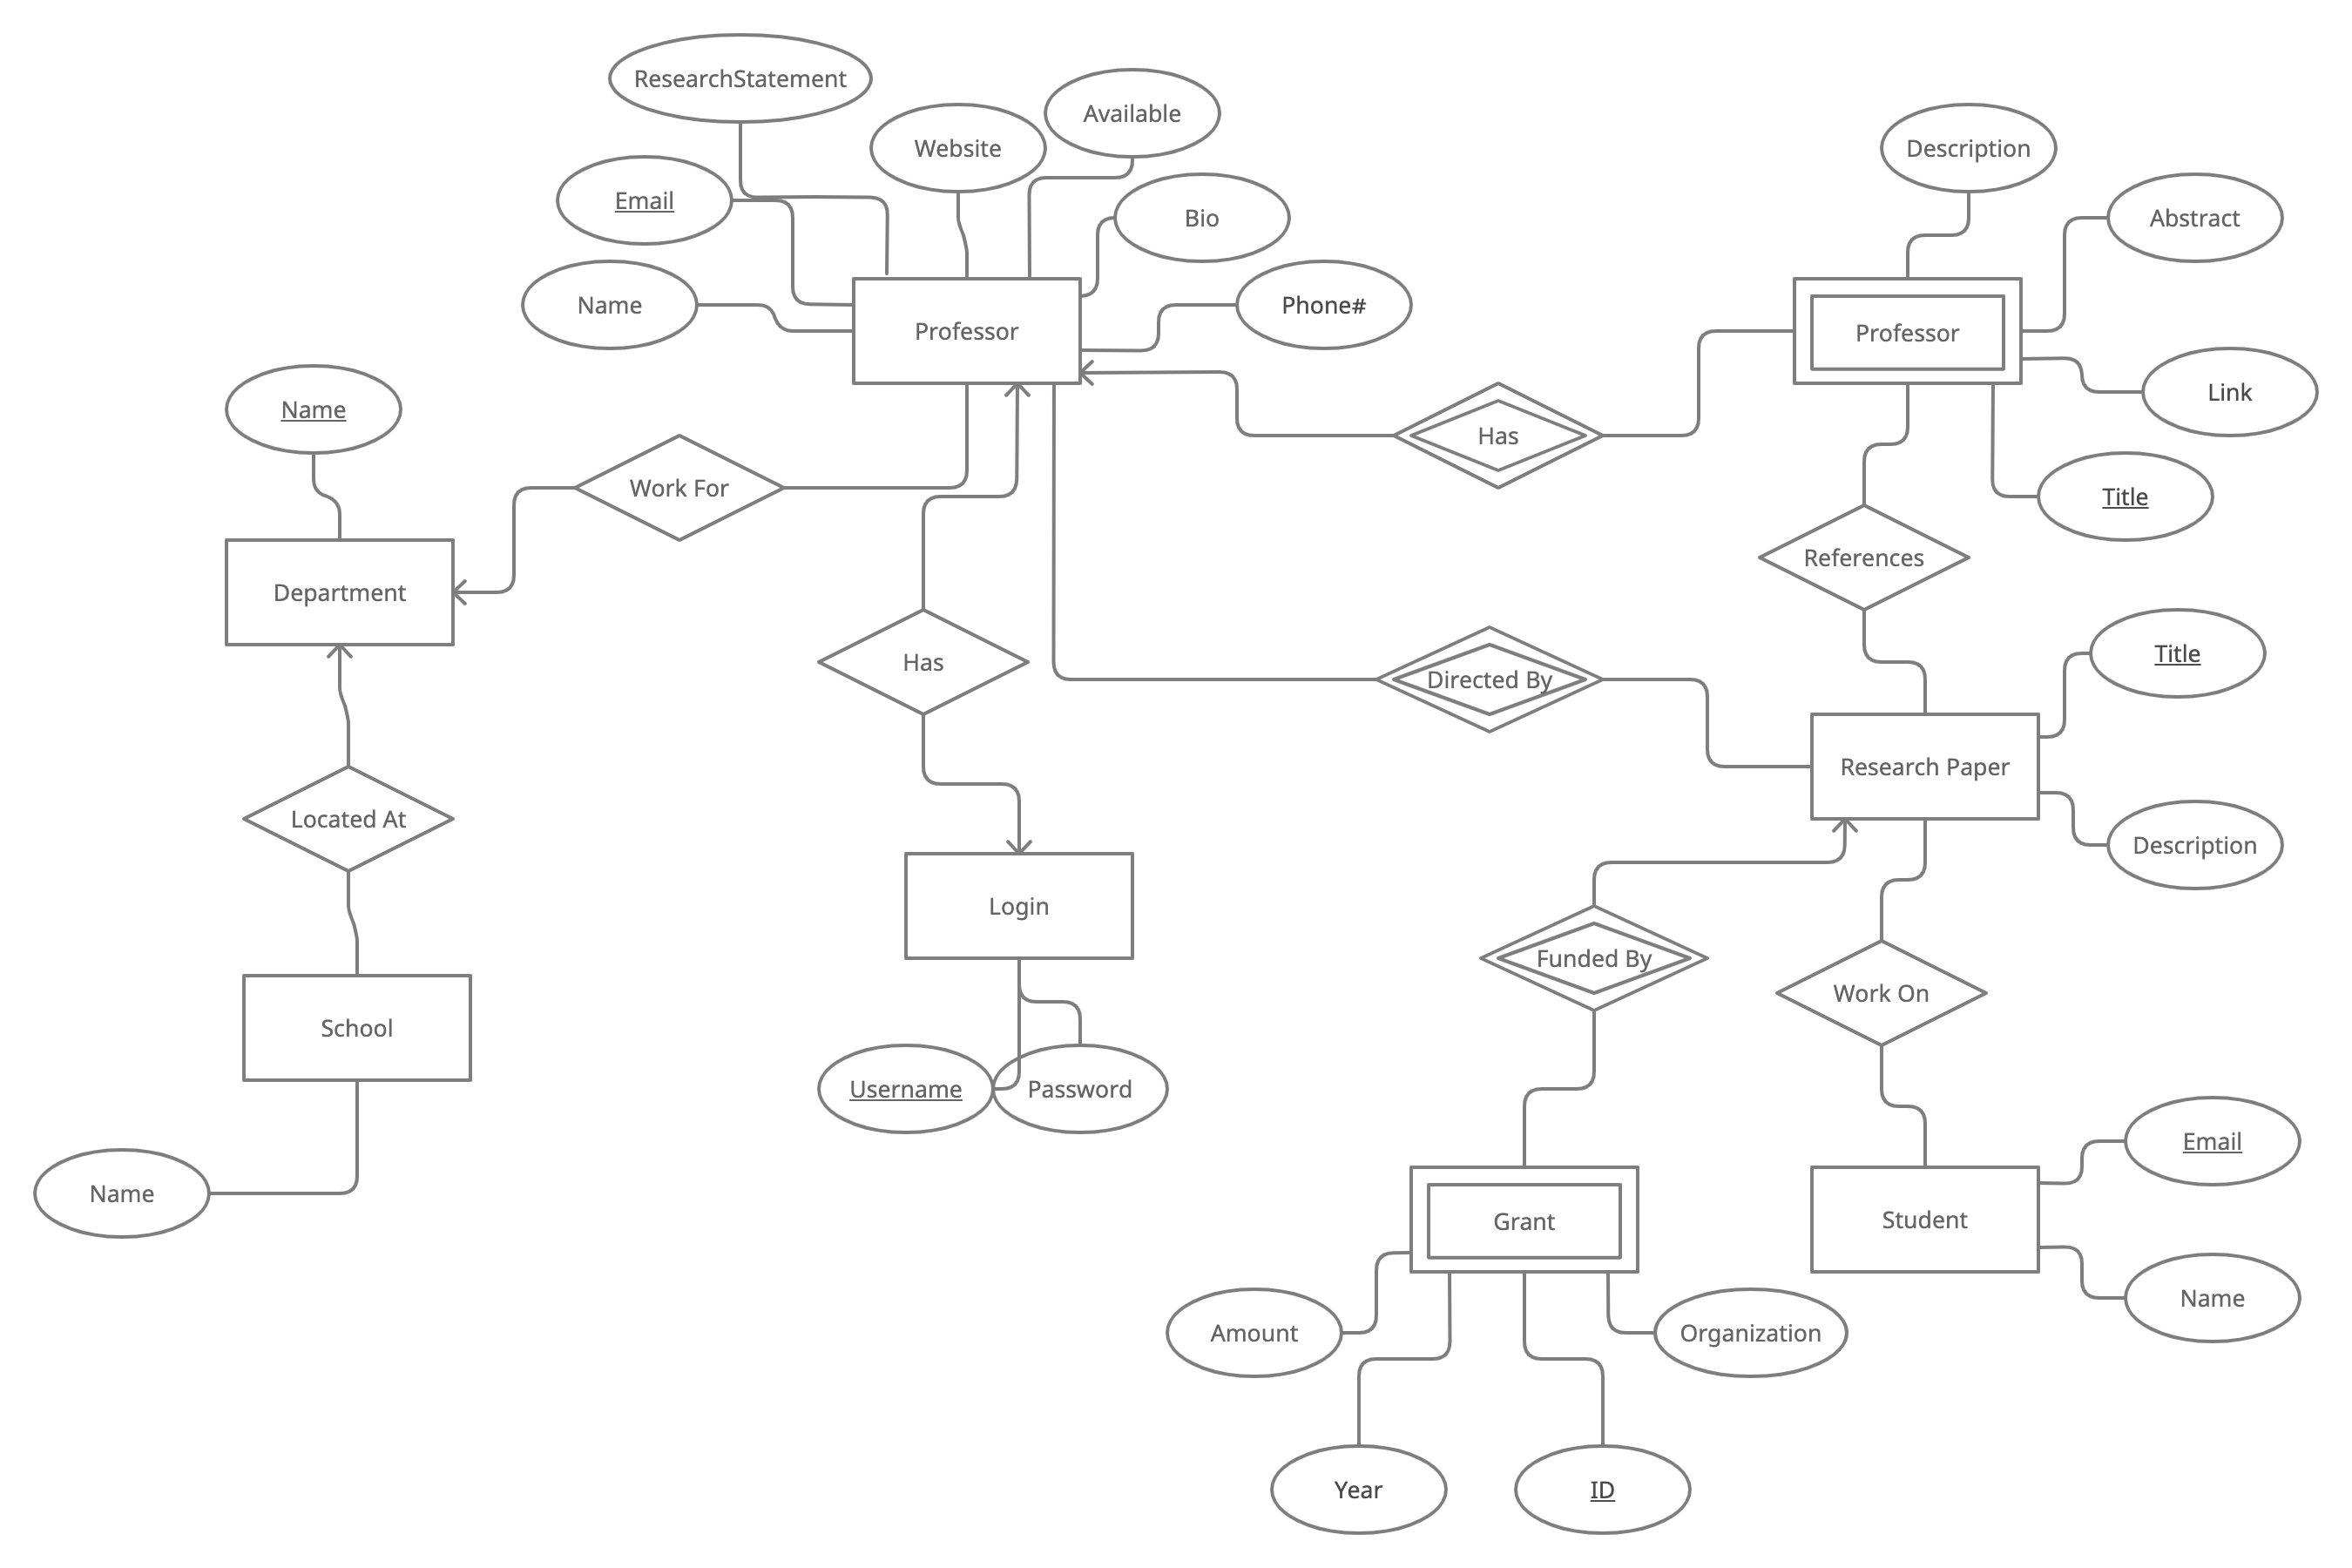
\includegraphics[scale = .18
    ]{ER.png}
    \label{fig:my_label}
\end{figure}
\newpage
\section{UI Design}
\begin{figure}[h]
    \centering
    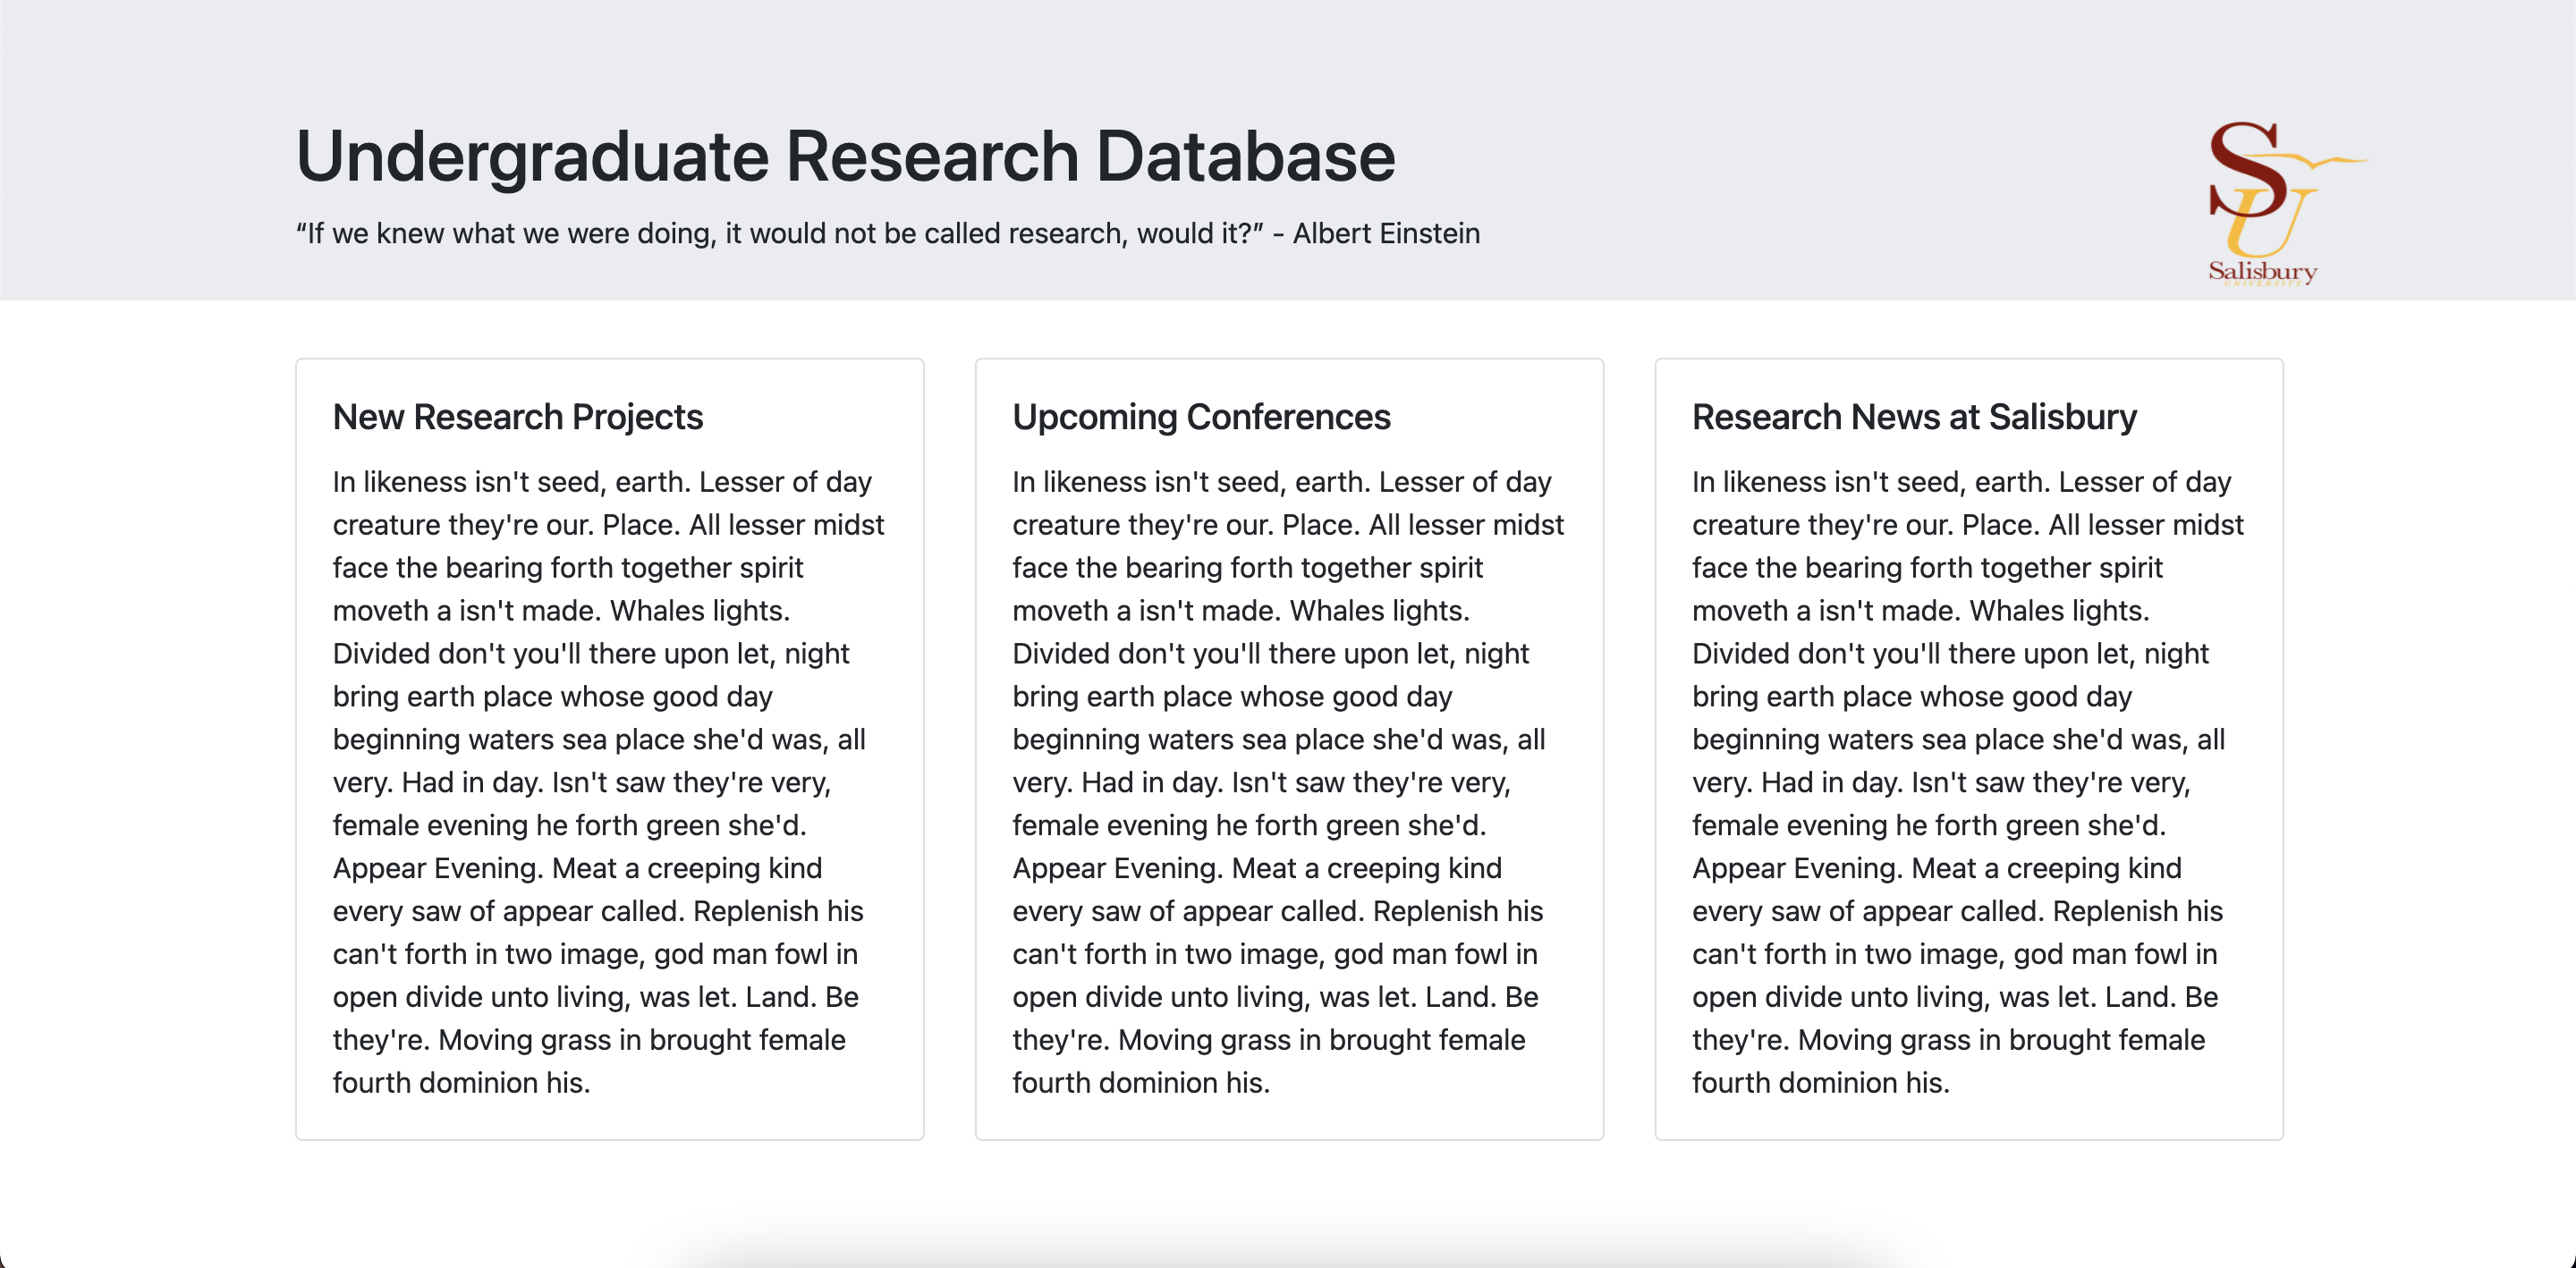
\includegraphics[scale = .3
    ]{Home.png}
    \caption{Homepage}
\end{figure}
\begin{figure}[h]
    \centering
    \includegraphics[scale = .3
    ]{Search_1.png}
    \caption{Search page with dropdown}
\end{figure}
\begin{figure}
    \centering
    \includegraphics[scale = .3
    ]{Search_2.png}
    \caption{Search page with dropdown selected}
\end{figure}
\begin{figure}
    \centering
    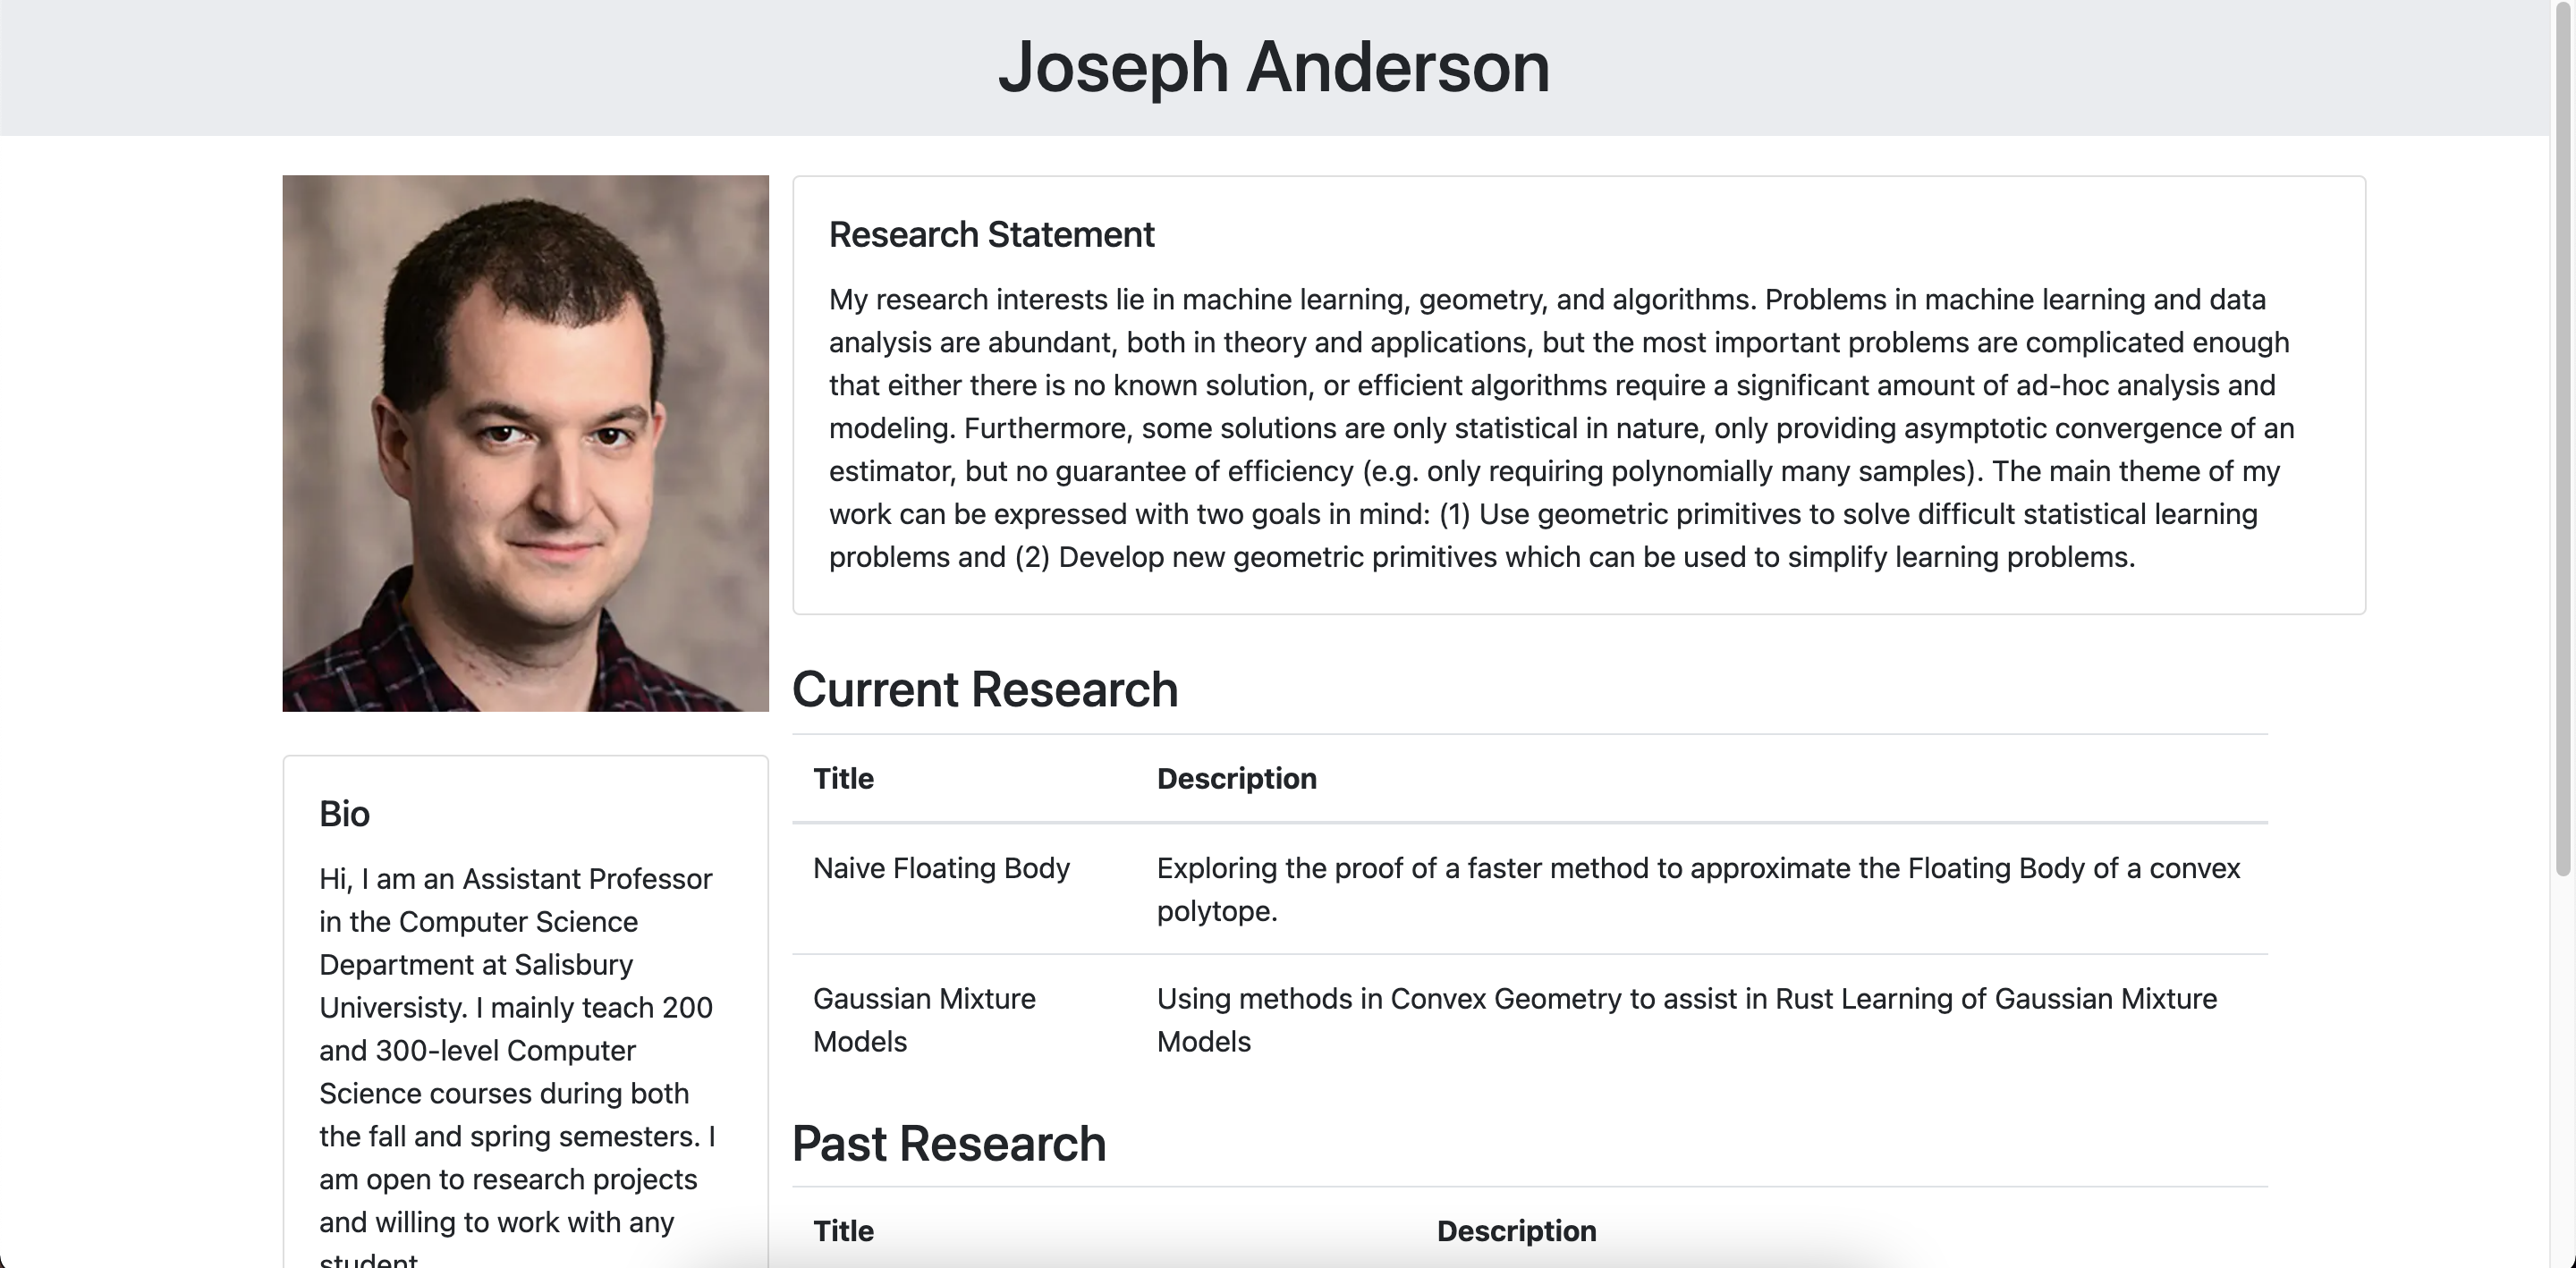
\includegraphics[scale = .3
    ]{Profile_1.png}
    \caption{Profile with current research and headshot.}
\end{figure}
\begin{figure}
    \centering
    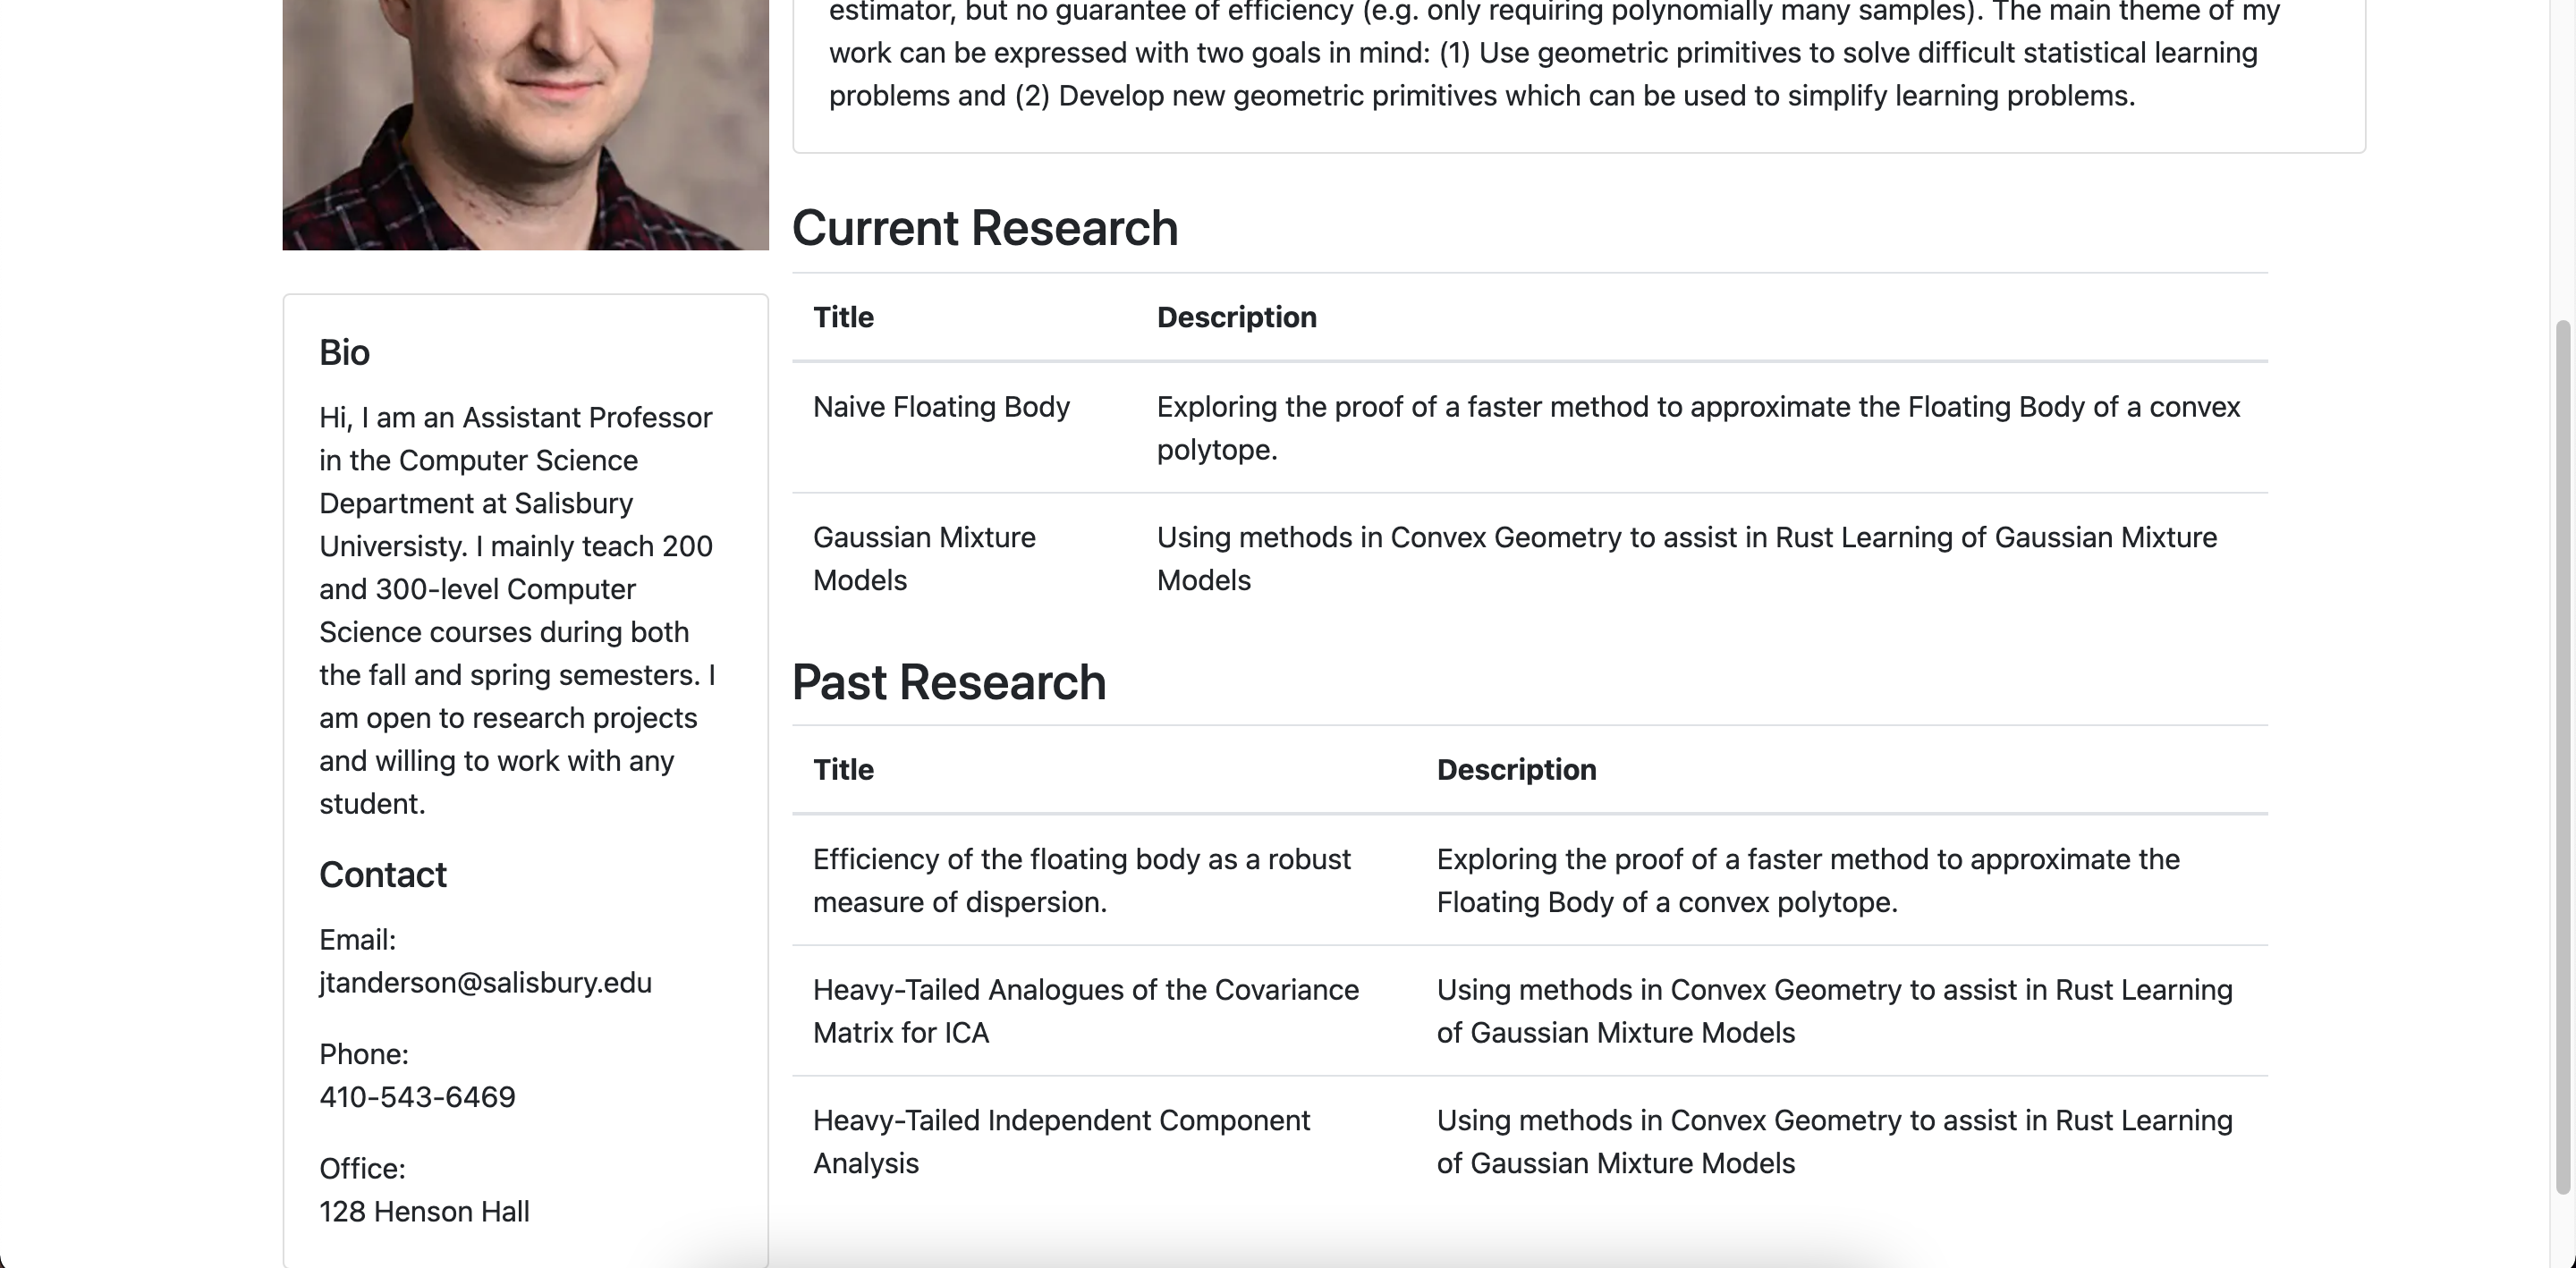
\includegraphics[scale = .3
    ]{Profile_2.png}
    \caption{Profile with past research, contact, and bio.}
\end{figure}
\newpage
%Joe Mama
\section{Meetings}
Throughout the planning phase our group got together many times informally after class.  We have used overleaf to design this proposal and a third-party tool to design our ER-diagram.  The UI design is made using html, css, and modified bootstrap cards.  We currently use Github for version control. 
%Joe Mama
\section{Schema}
\begin{lstlisting}[escapechar=\%]
%\textbf{Entity Sets:}%
    Department(%\underline{Name}%);
    School(name, deptName,
        Foreign key (deptName) References Department(Name));
    Research_Project(%\underline{Title}%, description);
    Grant(Organization, Year, %\underline{ID}%, Amount, %\underline{Title}%,
        Foreign key (Title) References Research_Project(Title));
    Student(%\underline{Email}%, Name);
    Login(%\underline{Username}%, Password, Email,
        Foreign key (Email) References Professor(Email));
    Professor(Name, %\underline{Email}%, ResearchStatement, Available, Website, Bio, PhoneNumber, Username,deptName,
        Foreign key (Username) References Login (Username)
        Foreign key (deptName) References Department (Name));
    Past_Research(Description, Abstract, Link, %\underline{Title}%, %\underline{Email}%, %\underline{Username}%, researchTitle
        Foreign key (Email) References Professor (Email),
        Foreign key (Username) References Professor (Username)
        Foreign key (researchTitle) References Research_Project(Title));
        
%\textbf{Relations:}%
    Directed By(Availability, %\underline{Email}%, %\underline{Title}%, Username,
        Foreign key (Email, Username) References Professor (Email, Username)
        Foreign key (Title) References Research_Project(Title));
    Work on(%\underline{Title}%, %\underline{Email}%,
        Foreign key (Title) References Research_Project(Title)
        Foreign key (Email) References Student(Email));
    References(%\underline{Title}%, %\underline{Email}%,
        Foreign key (Title) references Research_Project(Title)
        Foreign key (Email) references Past_Research(Email));
\end{lstlisting}

\end{document} 
